\documentclass[french,12pt,a4paper,titlepage]{report}
\usepackage[utf8]{inputenc}
\usepackage[T1]{fontenc}
\usepackage{babel}
\usepackage{graphicx}
\usepackage{hyperref}
\usepackage{nameref}
\title{Rapport projet base de données et PHP}
\author{Savinien Barbotaud, Ewen Piepers, François Jourden, Noan Perrot}
\begin{document}
	\maketitle
	
	% Page vide
	\newpage
	\thispagestyle{plain} % empty
	\mbox{}
    \addtocounter{page}{-1}
    \thispagestyle{empty}
    
	\tableofcontents
	\chapter{Préface}
	\section{Attendu de l'application}
	La réalisation attendue est une base de données liée à une application web permettant de gérer les relations entre l'université et les entreprises dans le cadre de contrats d'alternances et/ou de stages pour les étudiants, de contrats de vacataires, de donations ou encore de contrats entre les laboratoires rattachés à l'université et les entreprises.
	\section{Contraintes techniques}
	Nous avions pour contrainte l'utilisation du SGDB PostgreSQL ainsi que l'utilisation du langage de requête SQL et PLPGSQL pour programmer les déclencheurs de ce même SGDB.
	\newline
	De même, l'application web doit être codée en PHP dans sa version 8.2 sous le framework Slim-Skeleton en version 4. L'utilisation d'ORM extérieur est prohibé cependant la création d'un ne l'est pas.
	\section{Outils utilisés dans le développement de l'application}
	\paragraph{Base de données} PostgreSQL, PLPGSQL, PGAdmin, Python, DataGrip
	\paragraph{Application web} PHP, Slim Skeleton, Composer, Twig, AdminLTE, Bootstrap 4, TailwindCSS, PHPStorm, Visual Studio Code
	\paragraph{Développement} Docker (compose), Git, GitKraken, Git-LFS
	\chapter{Organisation}
	\section{Rôle dans l'équipe}
	\begin{table}[h]
		\centering
		\begin{tabular}{|l|l|}
			\hline
			\multicolumn{2}{|c|}{Membres de l'équipe} \\
			\hline
			PIEPERS Ewen & Responsable Git  \tabularnewline
			JOURDEN François & Responsable Base de données  \tabularnewline
			BARBOTAUD Savinien & Responsable UI/UX  \tabularnewline
			PERROT Noan & Chef d'équipe  \tabularnewline
			\hline
		\end{tabular}
		\caption{Nom et rôle de chaque participants}
	\end{table}
	\paragraph{Responsable Git}
	Chargé d'ordonner et de donner les directives sur l'utilisation dans Git des différentes branches, commits, fusions ainsi que de leur organisation.
	\paragraph{Responsable Base de données}
	Chargé de la création des vues, ainsi que des vérifications à l'insertion des données. Il vérifie également la conformité du schéma de définition des données avec la définition SQL de la base de données.
	\paragraph{Responsable UI/UX}
	Chargé du design des interfaces utilisateurs ainsi que des parcours utilisateurs. Il réalise également une partie du front-end et donne les directives à suivre en matière d'interface.
	\paragraph{Chef d'équipe}
	Coordonne les différents membres entre eux sur les tâches à effectuer. Il assiste les différents corps de métiers avec les technologies et aide au bon déroulement des tâches.
	\section{Établissement des tâches}
	La création des différentes tâches a commencé par une réflexion côté utilisateur de l'application. Notamment en partant des opérations qu'aurait besoin d'effectuer l'université sur les différentes représentations des données par le système d'information. De cette réflexion a pu en découler différentes épic et story utilisateur que nous avons représenté sous forme de tickets en adoptant la pratique de gestion de projet AGILE.
	\newline
	\newline
	La création des ticket s'est faite en utilisant GitLab, le même outil qui gère nos version de code afin de simplifier le workflow de l'équipe en minimisant le nombre d'outils à utiliser. De plus, l'équipe s'était déjà familiarisée avec cet outil lors de précédents projets personnels et/ou professionnels.
	\newline
	\begin{figure}[ht]
		\centering
		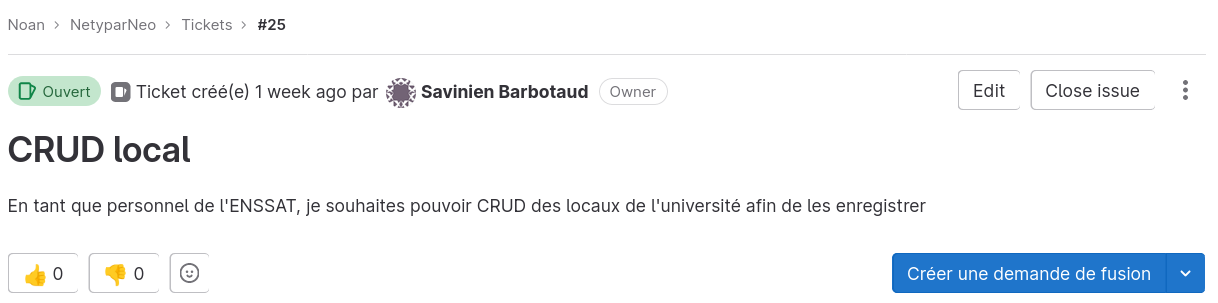
\includegraphics[width=0.7\linewidth]{rapports_assets/screenshot001}
		\caption{Exemple de tickets créés}
		\label{fig:screenshot001}
	\end{figure}
	\newline
	Pour les états des différents tickets nous avons adopté l'approche Kanban. Chaque ticket à un état: A faire, en cours, terminé. Cela permet d'indiquer aux autres participants sur le projet leur avancement de manière simple et claire sur une tâche.
	\newline
	\begin{figure}[ht]
		\centering
		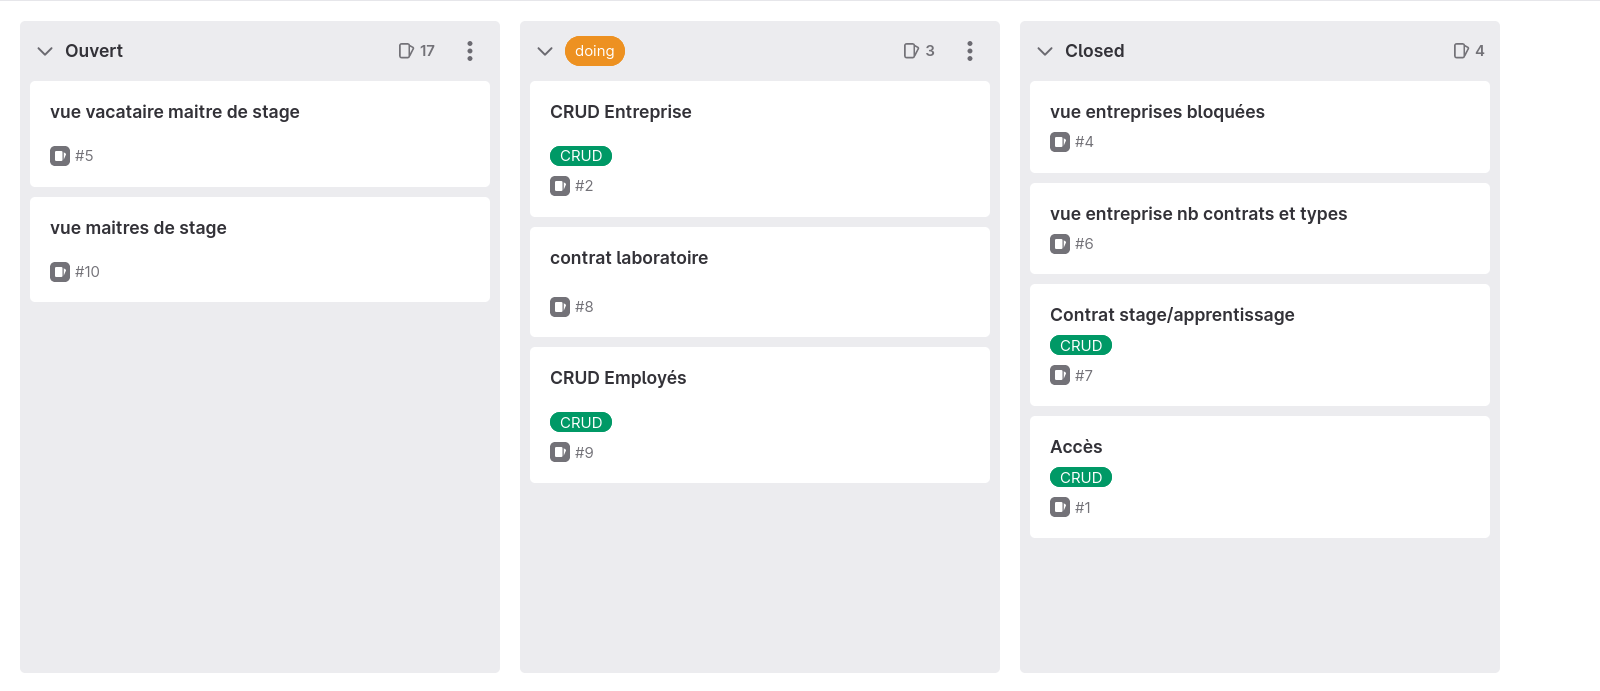
\includegraphics[width=0.7\linewidth]{rapports_assets/screenshot002}
		\caption{Tableau Kanban dans le cadre du projet}
		\label{fig:screenshot002}
	\end{figure}
	\newline
	Nous avons choisi de ne pas faire de report de temps sur les différentes tâches. En effet, il était compliqué pour nous de suivre le temps passé sur chaque tâches comme certaines pouvait durée moins d'une heure à être réalisé ou certaine nécessitait d'être en continuel développement pendant tout le projet. De plus, nous n'avons pas connaissance d'outils de suivi de temps et le projet n'ayant pas une échéance de rendu longue, son utilisation nous paraissait peut pertinente dans le cadre de ce projet.
	\section{Git}
	Pour l'organisation du GIT, nous nous sommes inspirés du workflow vu en entreprise à savoir : 
	\paragraph{Branche master}
	Cette branche n'est ni une branche de développement, ni de debug. Elle contient les versions du projet
	\paragraph{Branche develop}
	Est une branche d'intégration. Les features qui ont été développées sont mise en relation pour tester leur bon fonctionnement.
	\paragraph{Feature}
	Toutes les autres branches sont des améliorations de develop, ou la création de feature sur le projet.
	\begin{figure}[ht]
		\centering
		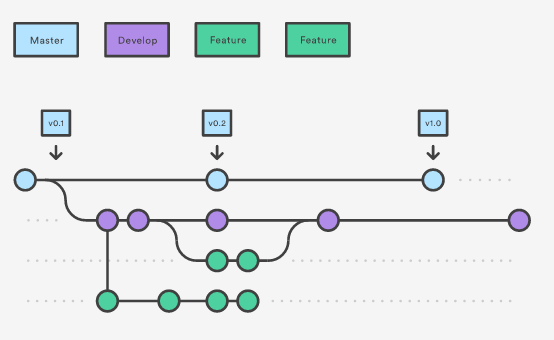
\includegraphics[width=1\linewidth]{rapports_assets/git_flow.png}
		\caption{Les différentes tables et leurs relations identifiées dans la base de données}
	\end{figure}
	\chapter{Conception}
		\section{Base de données}
		Nous avons commencé par concevoir la base de données de l'application.
		\newline
		Pour ce faire, nous avons choisis un méthode consistant à effectuer plusieurs passages ensembles sur le sujet donné afin d'y identifier les différents besoins couche par couche.
		\subsection{Objets} Nous avons commencé par identifier les différents objets sous forme de table que nous aurions à retrouver dans notre base de données.
		\newline
		\begin{figure}[ht]
			\centering
			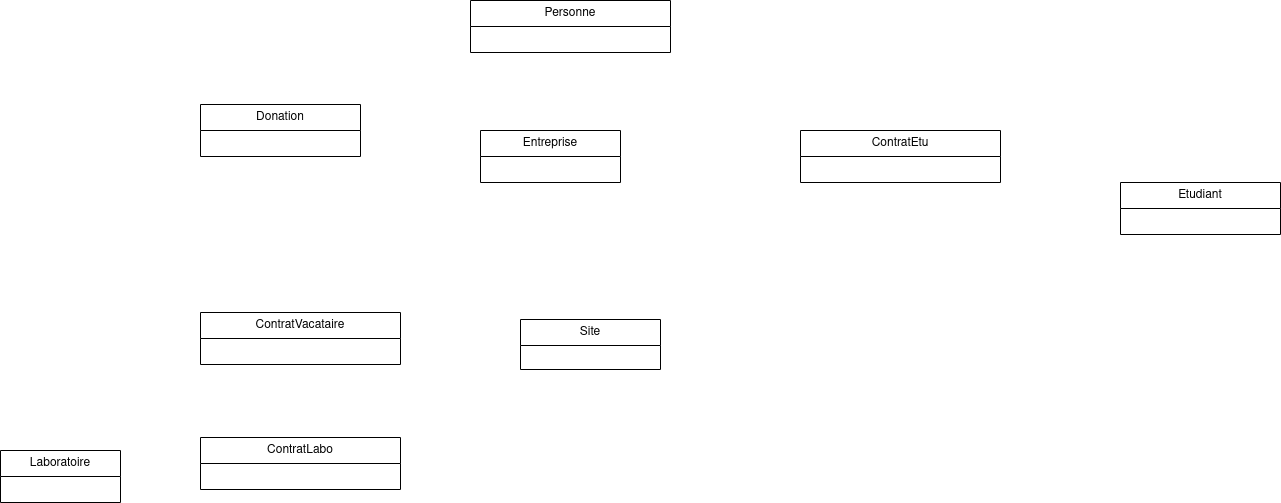
\includegraphics[width=1\linewidth]{rapports_assets/diag_db_table_only.png}
			\caption{Les différentes tables identifiées dans la base de données}
		\end{figure}
		\newline
		Ici, nous avons séparés les différentes formes de contrats sous la forme des contrats vacataires, contrats etudiants (stage et alternance) et donations à cause de leurs différent jeux de donnés que nous verrons plus tard.
		\newline
		Nous avons réunis les tables vacataire et maitre de stage car celle-ci représentaient la même chose : des personnes travaillant pour des entreprises avec les mêmes informations.
		\subsection{Les Relations} Nous avons ensuite cherché à comprendre comment ces différentes tables étaient liées entre elles dans notre base de données.
		\newline
		\begin{figure}[ht]
			\centering
			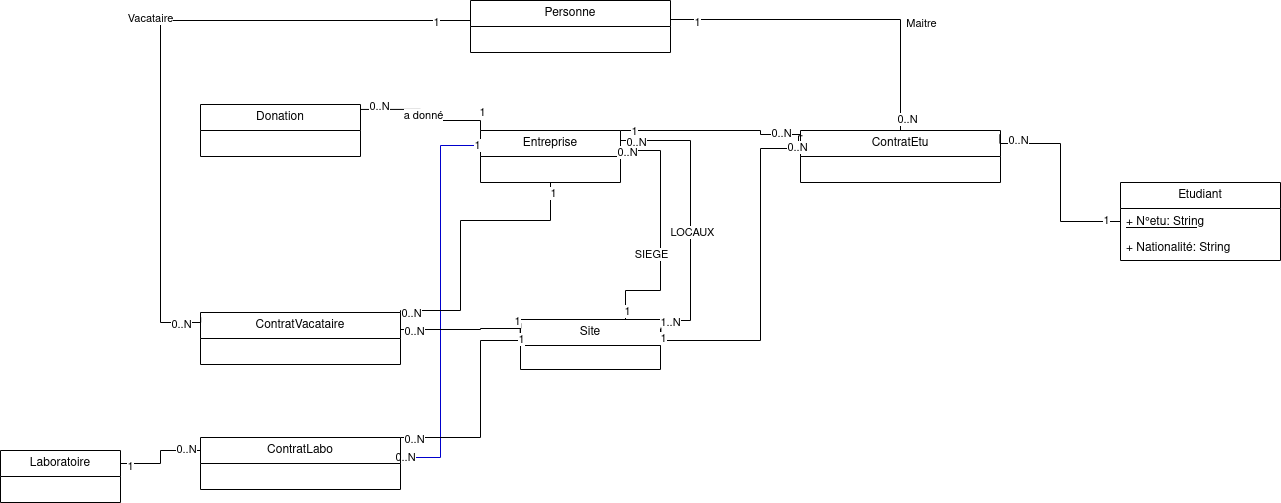
\includegraphics[width=1\linewidth]{rapports_assets/diag_db_table_relation.png}
			\caption{Les différentes tables et leurs relations identifiées dans la base de données}
		\end{figure}
		\newline
		Les deux relations \textit{Siege} et \textit{Locaux} représentent ici les différents possibles liens que peut avoir une entreprise avec un site, qui peut donc être soit le siège de cette entreprise soit un simple local de celle-ci.
		\newline
		Nous aurions pu simplement créer une relation Entreprise(1)--(1..N)Site, mais celle-ci était contraignante dans le sens où
		\begin{itemize}
		\item Cela nous obligeais à créer une relation 1-1, qui est une chose irréalisable en SQL
		\item Cela contraignait nos sites à une seule entreprise, mais il existe par exemple des locaux partagés par plusieurs entreprise (chose que nous avons confirmée avec le professeur)
		\end{itemize}
		Nous avons également pris la décision de ne pas indiquer directement la relation entre les tables \textit{Personne} et \textit{Entreprise} pour la simple raison que nous n'avons pas réellement besoin de cette information, les contrats étudiants suffisent à donner l'appartenance d'une personne à un moment donné, et cela représenterait une charge de travail inutile et fastidieuse pour l'utilisateur de l'application finale.
		\subsection{Les attributs}
		Enfin, nous nous sommes attelés à chercher dans le sujet tous les attributs que nous devions retrouver dans nos tables.
		\begin{figure}[ht]
			\centering
			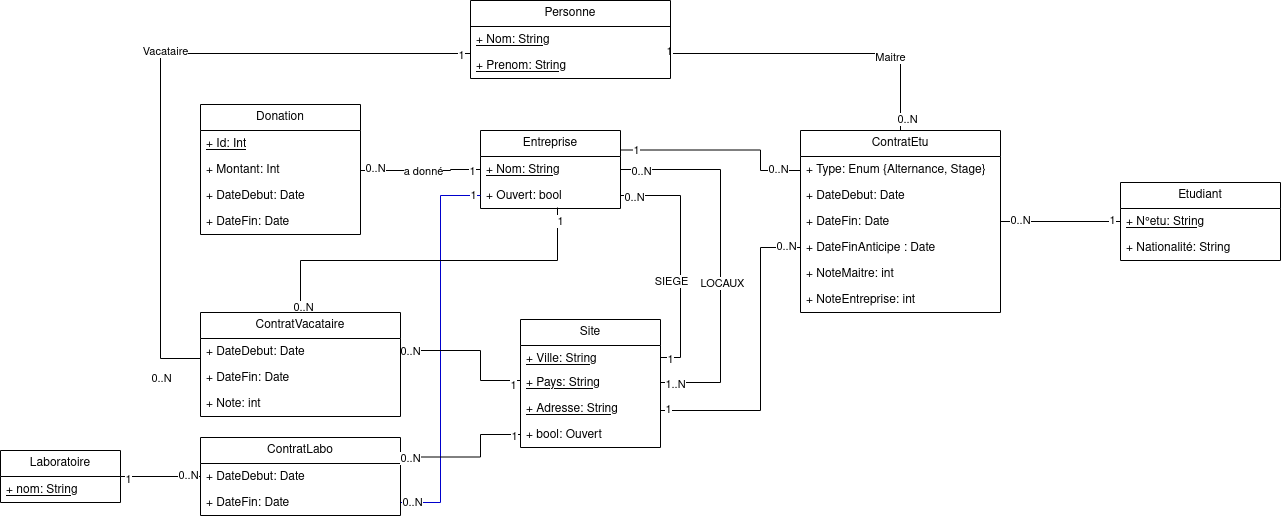
\includegraphics[width=1\linewidth]{rapports_assets/diag_db_complete.png} 
			\caption{Les différentes tables, leurs relations et leurs attributs}
		\end{figure}
		Pour les contrats étudiants, nous avons simplement choisi un attribut de type enum, avec les valeurs \textit{stage} et \textit{alternance} afin de différencier ces deux types de contrat qui comportent les mêmes attributs.
		\newline
		Nous avons également veillé à donner les mêmes nom aux attributs communs de toutes \textbf{les tables de contrat} (\textit{donation}, \textit{contrat de laboratoire} et \textit{Contrat étudiant}) afin de faciliter d'éventuels unions entre ces tables

		\subsection{La base de données} (fig 3.4)
	Au final, nous avons ajouter quelques tables et clés étrangères pour  créer ces relations.
	\clearpage
		\begin{figure}[ht]
			\centering
			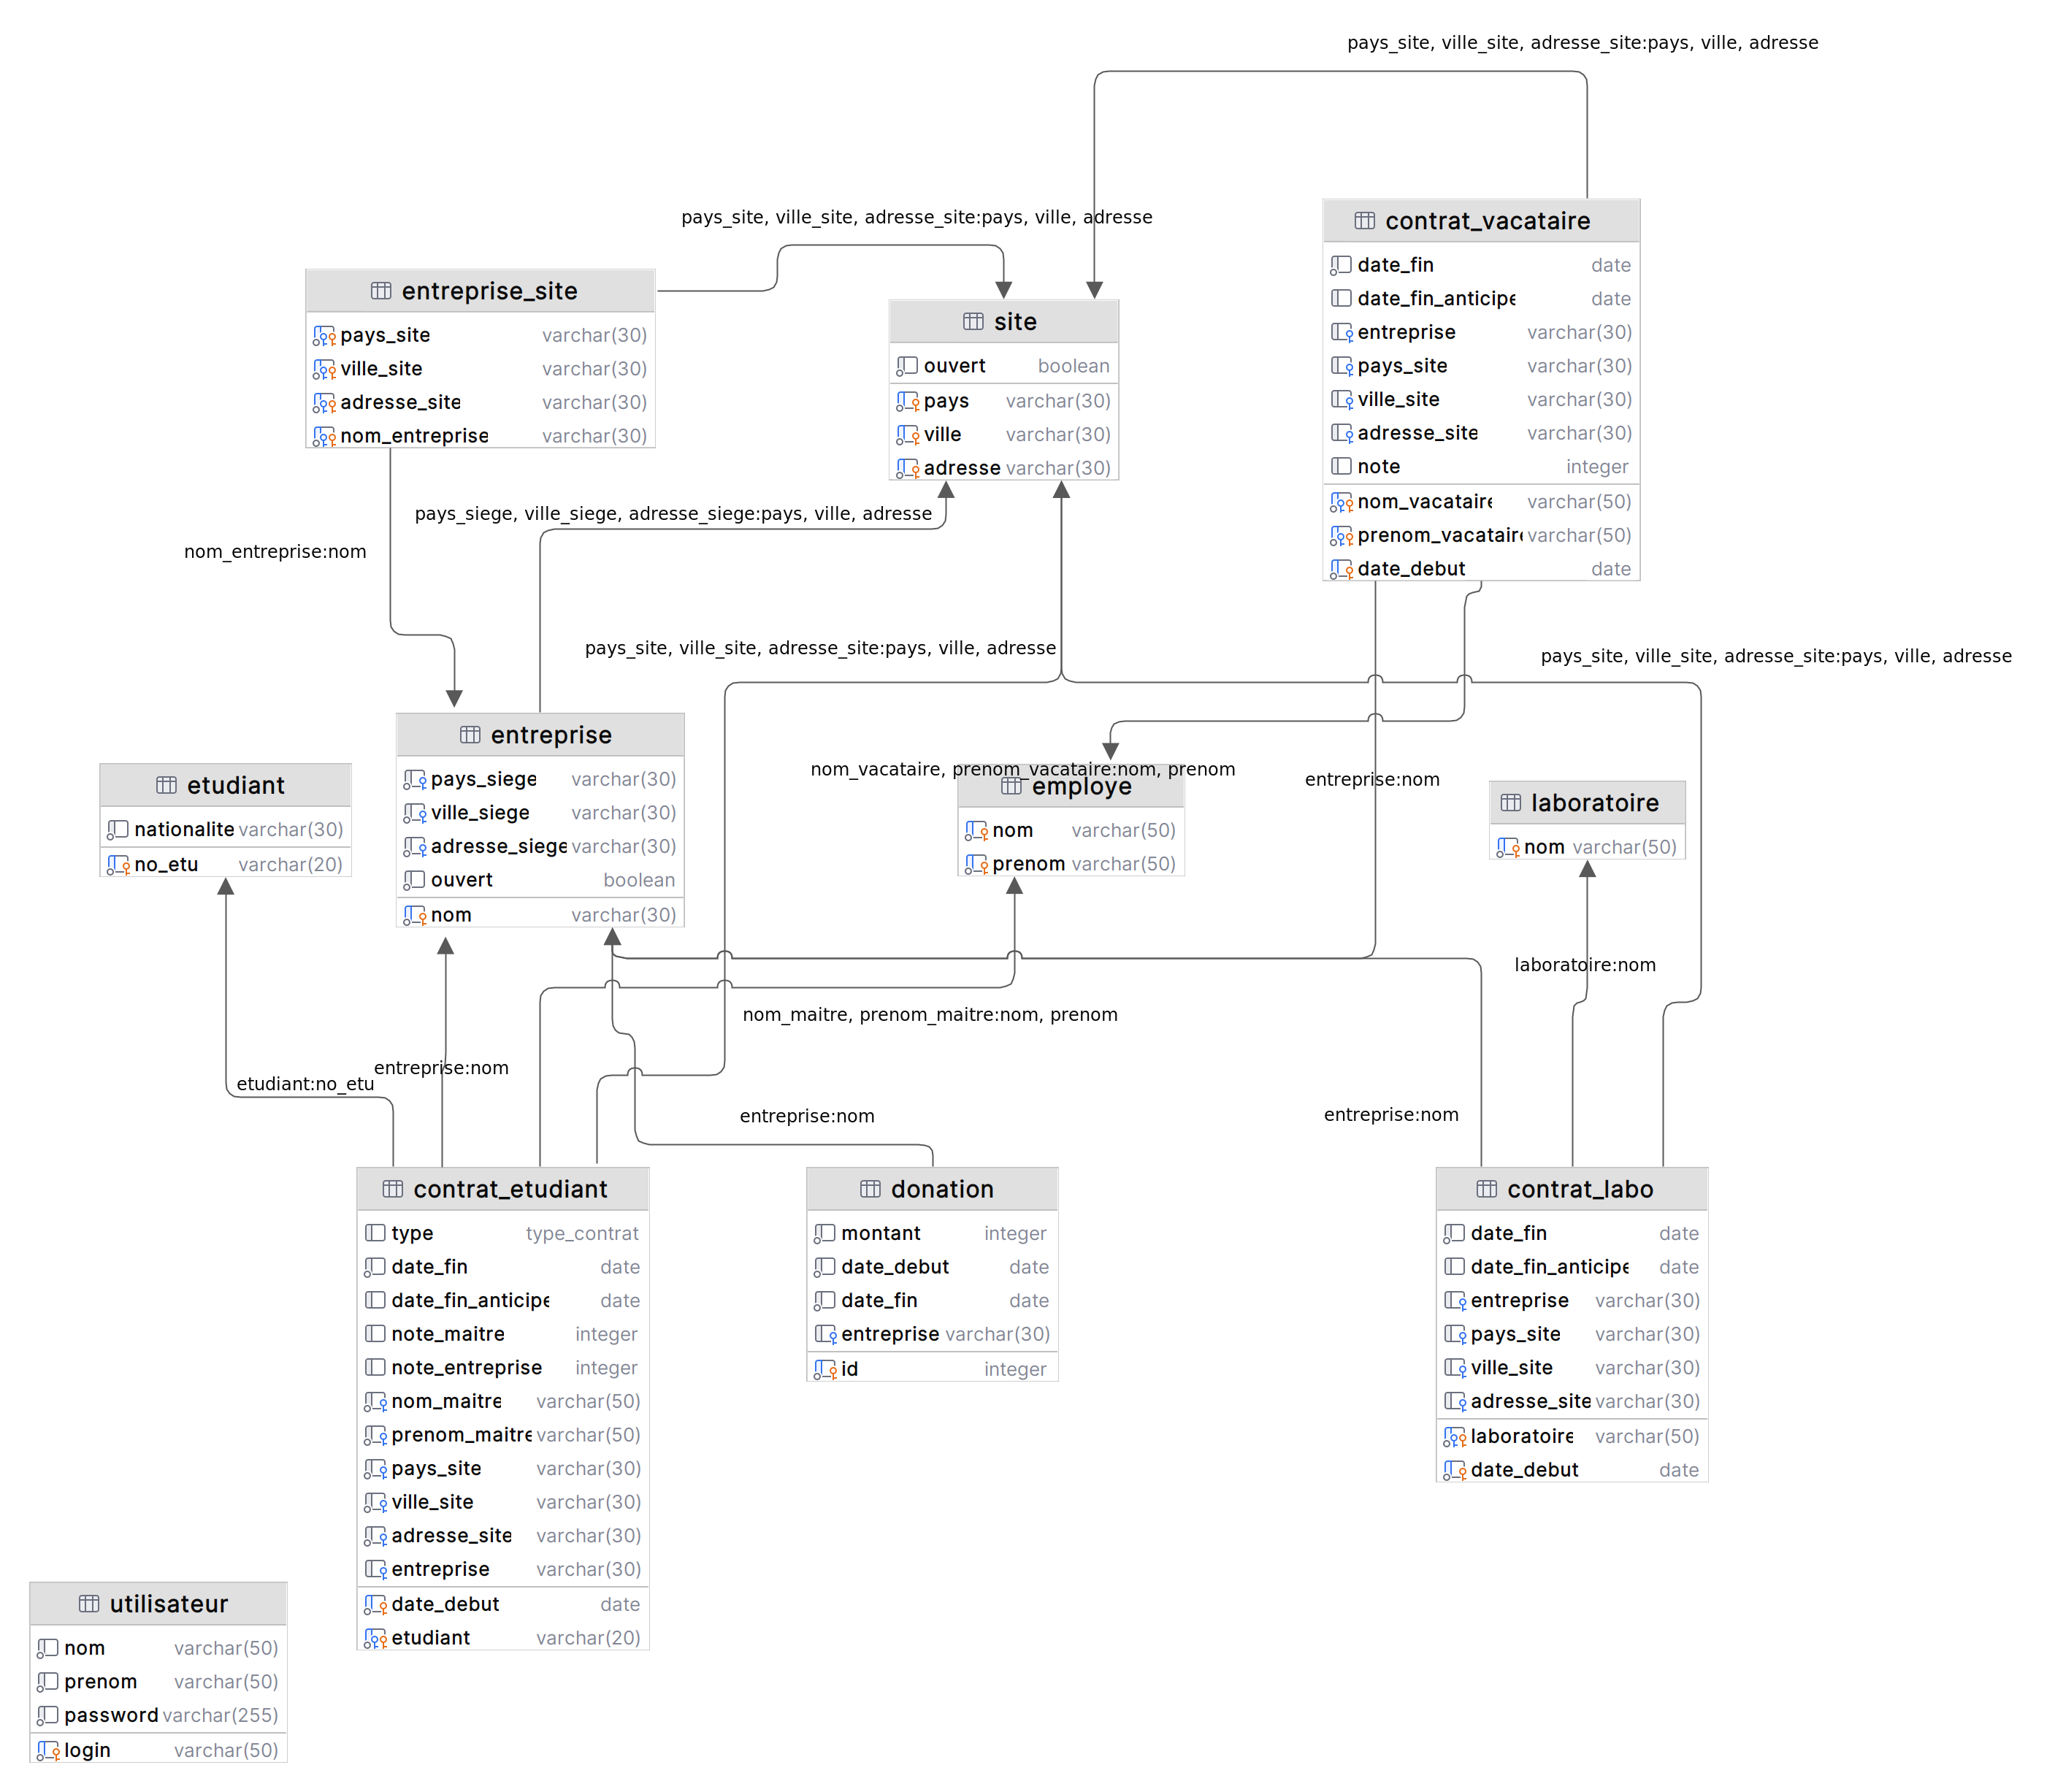
\includegraphics[width=1\linewidth]{rapports_assets/diag_table_complete.png} 
			\caption{Les différentes tables, leurs attributs et leurs clés étrangère}
		\end{figure}
		Nous avons ici ajouter une table \textit{entreprise\_site} qui nous sert à enregistrer la relation entre les entreprises et leurs locaux.
		\newline
		Nous avons également mis en place une table \textit{utilisateur} nous permettant de stocker les utilisateurs de l'application, avec un mot de passe qui sera hash côté application en PHP.
		Nous avons également fait le choix de mettre certains attributs en \textit{nullable} ou en \textit{not null}, selon les besoin. On peut distinguer un point en bas à gauche du logo de chaque attribut \textit{not null}

		\section{Application}

		\subsection{Modèles de l'application}
		Enfin, nous avons créer nos classes de modèle dans l'application.
		\newline
		\begin{figure}[ht]
			\centering
			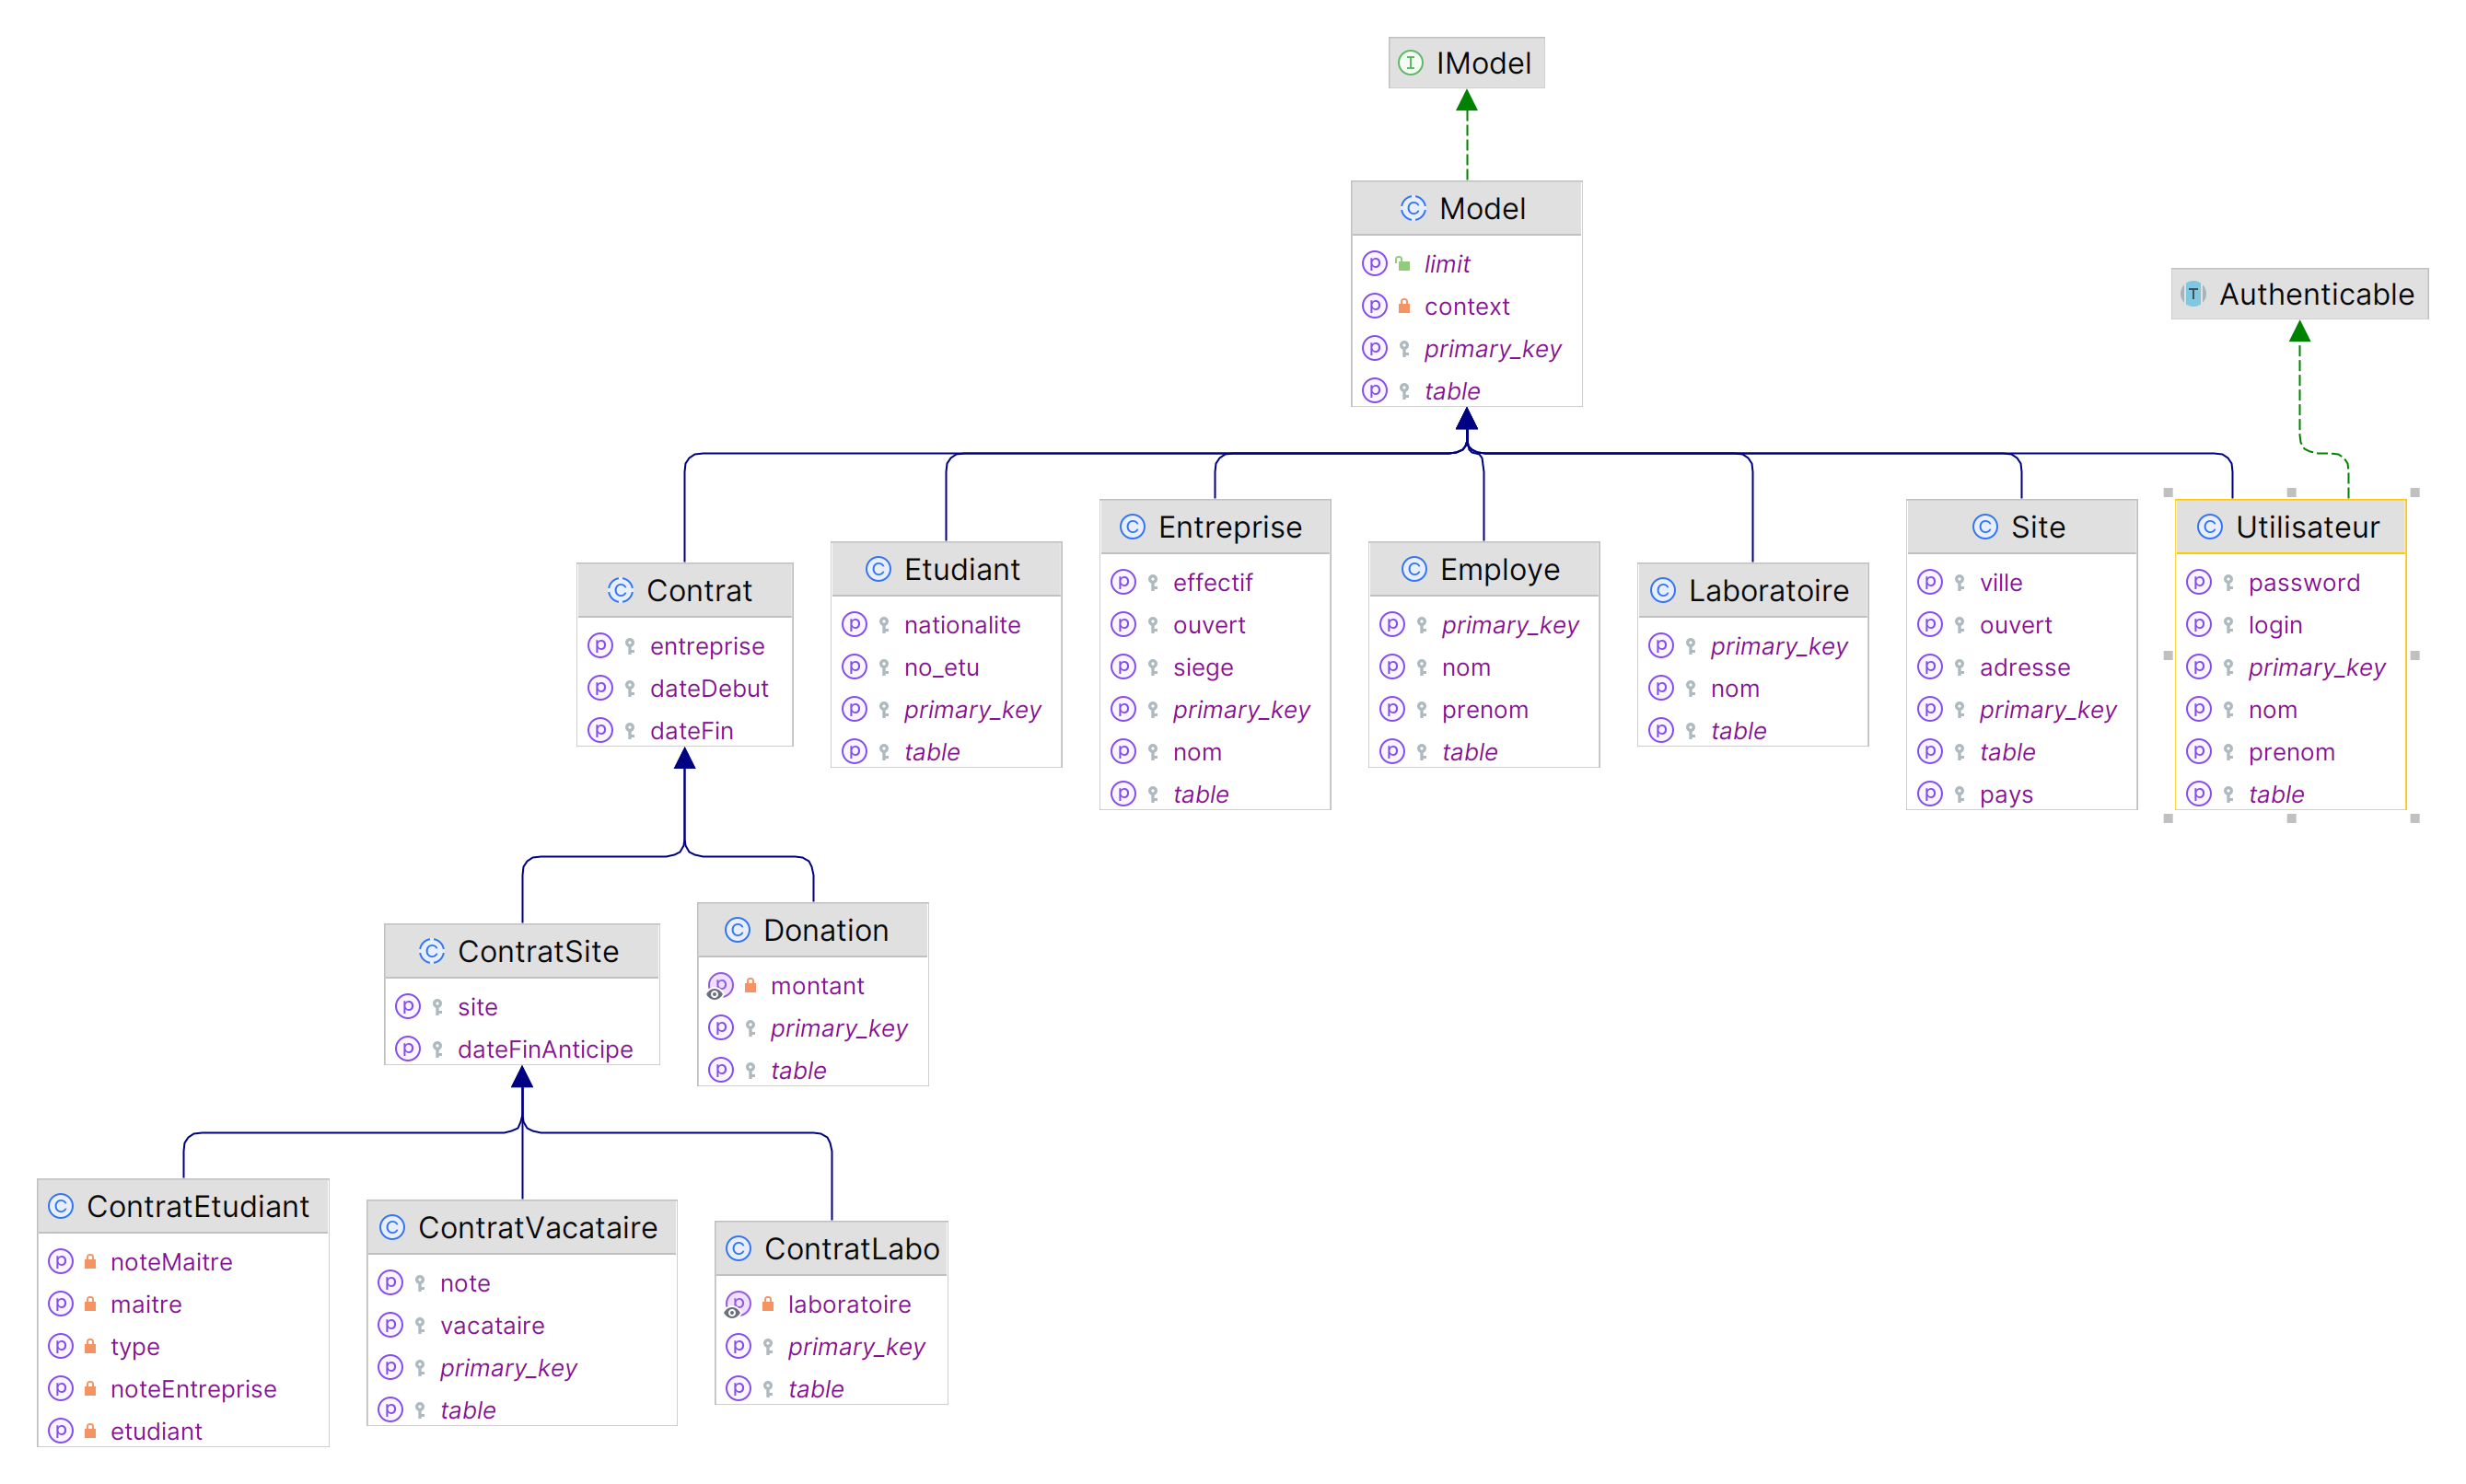
\includegraphics[width=1\linewidth]{rapports_assets/app_model_classes.png} 
			\caption{Les différentes tables identifiées dans la base de données}
		\end{figure}
		\newline
		Nous avons basé tous nos modèles sur une classe abstraite \textit{Model} qui nous permet de créer un ORM que nous verrons plus en détail dans la partie Application.
		\newline
		Nous avons également fait le choix, concernant les contrats de les faire tous hériter d'une classe \textit{Contrat} qui regroupe leurs champs communs, puis d'une classe \textit{ContratSite} pour les contrats liés à un site.
		\subsection{Docker et Docker-Compose}
		Lors du développement de l'application web, nous avons été confronté à une problématique qui était: "Comment être sûr de développer sur les mêmes environnements ?". En effet, un développeur sous ArchLinux n'aura pas la même version de PHP qu'un sur Ubuntu ou sur Mint. Cela est d'autant plus dangereux que Composer (gestionnaire de dépendances pour PHP) peut introduire des incompatibilités de librairies selon la version de PHP et l'environnement de chaque développeur. Il nous fallait une solution que chaque développeur est une environnement ISO les uns des autres.
		\newline
		Nous avons opté pour l'utilisation de Docker nous permettant d'avoir une base de donnée PostgreSQL lié à un serveur PHP tout deux monolithique sur leur version et configuration permettant aux développeurs d'être tous sur le même environnement. Pour cela, l'utilisation de Docker Compose fu très utile car cet outil permet de créer des containers en les inter-connectant et orchestrant de manière simple et rapide.
		\subsection{Model View Controller}
		L'architecture adopté pour la réalisation de l'application web est MVC. Ce choix c'est fait pour plusieurs raisons, la première est que le framework que nous utilisons (Slim Skeleton) intègre déjà cette architecture. La seconde est que notre équipe est déjà formé à cette architecture grâce aux cours de Web mais aussi aux divers projets qu'ils ont pu mener.
	\chapter{Développement}
	\section{Base de données}
	\subsection{Trigger} 
	Afin de répondre à la contrainte du projet notifiant qu'une entreprise ne peut avoir que trois stagiaires et/ou alternant à la fois si sa masse salariale est inférieure à 20 sinon elle ne peut avoir pas plus de 15\% de sa masse salariale en contrat d'alternance ou de stage, nous avons créer un trigger.
	
	Ce trigger utilise deux fonctions, une fonction permettant de récupérer les contrats d'alternances ou de stage d'une entreprise, la seconde, utilisant la première, permet de déterminer en fonction de la masse salariale d'une entreprise si elle peut accueillir un nouvel apprenti ou stagiaire. 
	
	\subsection{Contraintes diverses}
	Dans le but d'assurer la cohérence de la base de données, nous avons inclu plusieurs contraintes de type check. Notement pour s'assurer que les dates de début des contrats n'étaient pas après les dates de fin. Nous nous en sommes aussi servi afin de vérifier que les montants des donations n'étaient pas négatifs ou encore que les notes étaient bien comprises entre 0 et 10.
	 
	\section{Application}
	\subsection{CRUD}
	\paragraph{Définition} CRUD pour Create, Read, Update, Delete. Désigne les 4 opérations de base pour la persistance des données
	\paragraph{Mise en place} Dans le ficher de routes, les différents modèles sont regroupés pour établir les contraintes CRUD
	\subsection{Twig, gestion des vues et adminLTE}
	\paragraph{adminLTE} AdminLTE est une solution open source permettant de créer des dashboards simple à l'aide de bootstrap. L'organisation dans les vues Twig est régis pas adminLTE
	\paragraph{Choix de l'architecture} Toutes les pages du site possèdent un header ainsi que la sidebar. \newline 
	Afin de ne pas modifier toutes les vues à chaque ajout de page, ces deux composants ont été séparés et implémentés dans chaque vue.
	\newline
	Les importations des différentes ressources comme tableur-icon ou les librairies JS ont été un problème car différentes dans chaque pages. De ce fait, un template a été créé, importé dans chaque page, seul le contenu de la page peut être modifié. 
	\subsection{Debug bar}
	\paragraph{Contexte}
	La debug bar est un outil pour le développement de sites web dynamiques. Cet outil peut indiquer les erreurs des vues, les paramètres passés par le controller, les routes empruntées, et même encore les requêtes effectuées sur la base de donnée.
	\paragraph{Utilisation}
	Par manque de temps, nous avons utilisé une debug bar existante. Nous avons choisi celle de MaximeBF sur github, pour sa compatibilité avec le framework slim et les vues Twig. Installée 58 Millions de fois est un gage de bon fonctionnement et la possibilité d'avoir les questions de la communauté en cas de problème.
	\newline
	\textbf{\href{https://github.com/maximebf/php-debugbar}{Github debug bar}}
	\paragraph{Intégration}
	Les paramètres du container slim indique si la debug bar doit être présente ou non. Dans le cas positif, elle est ajoutée avant la compilation ou le rendu d'un template.
	\chapter{Conclusion}
	\listoffigures
	\listoftables
\end{document}